%% Curriculum vitæ inséré depuis un fichier PDF externe
\clearpage

%% mise en page commune à toutes les pages insérées :
%% style « plain » (folio seul, comme les pages de début de chapitre),
%% page insérée réduite et remontée pour ne pas empiéter sur le pied de page
\newcommand{\cvpagestyle}{\thispagestyle{plain.scrheadings}}

%% première page : ajout de l'entrée dans la table des matières et des signets PDF
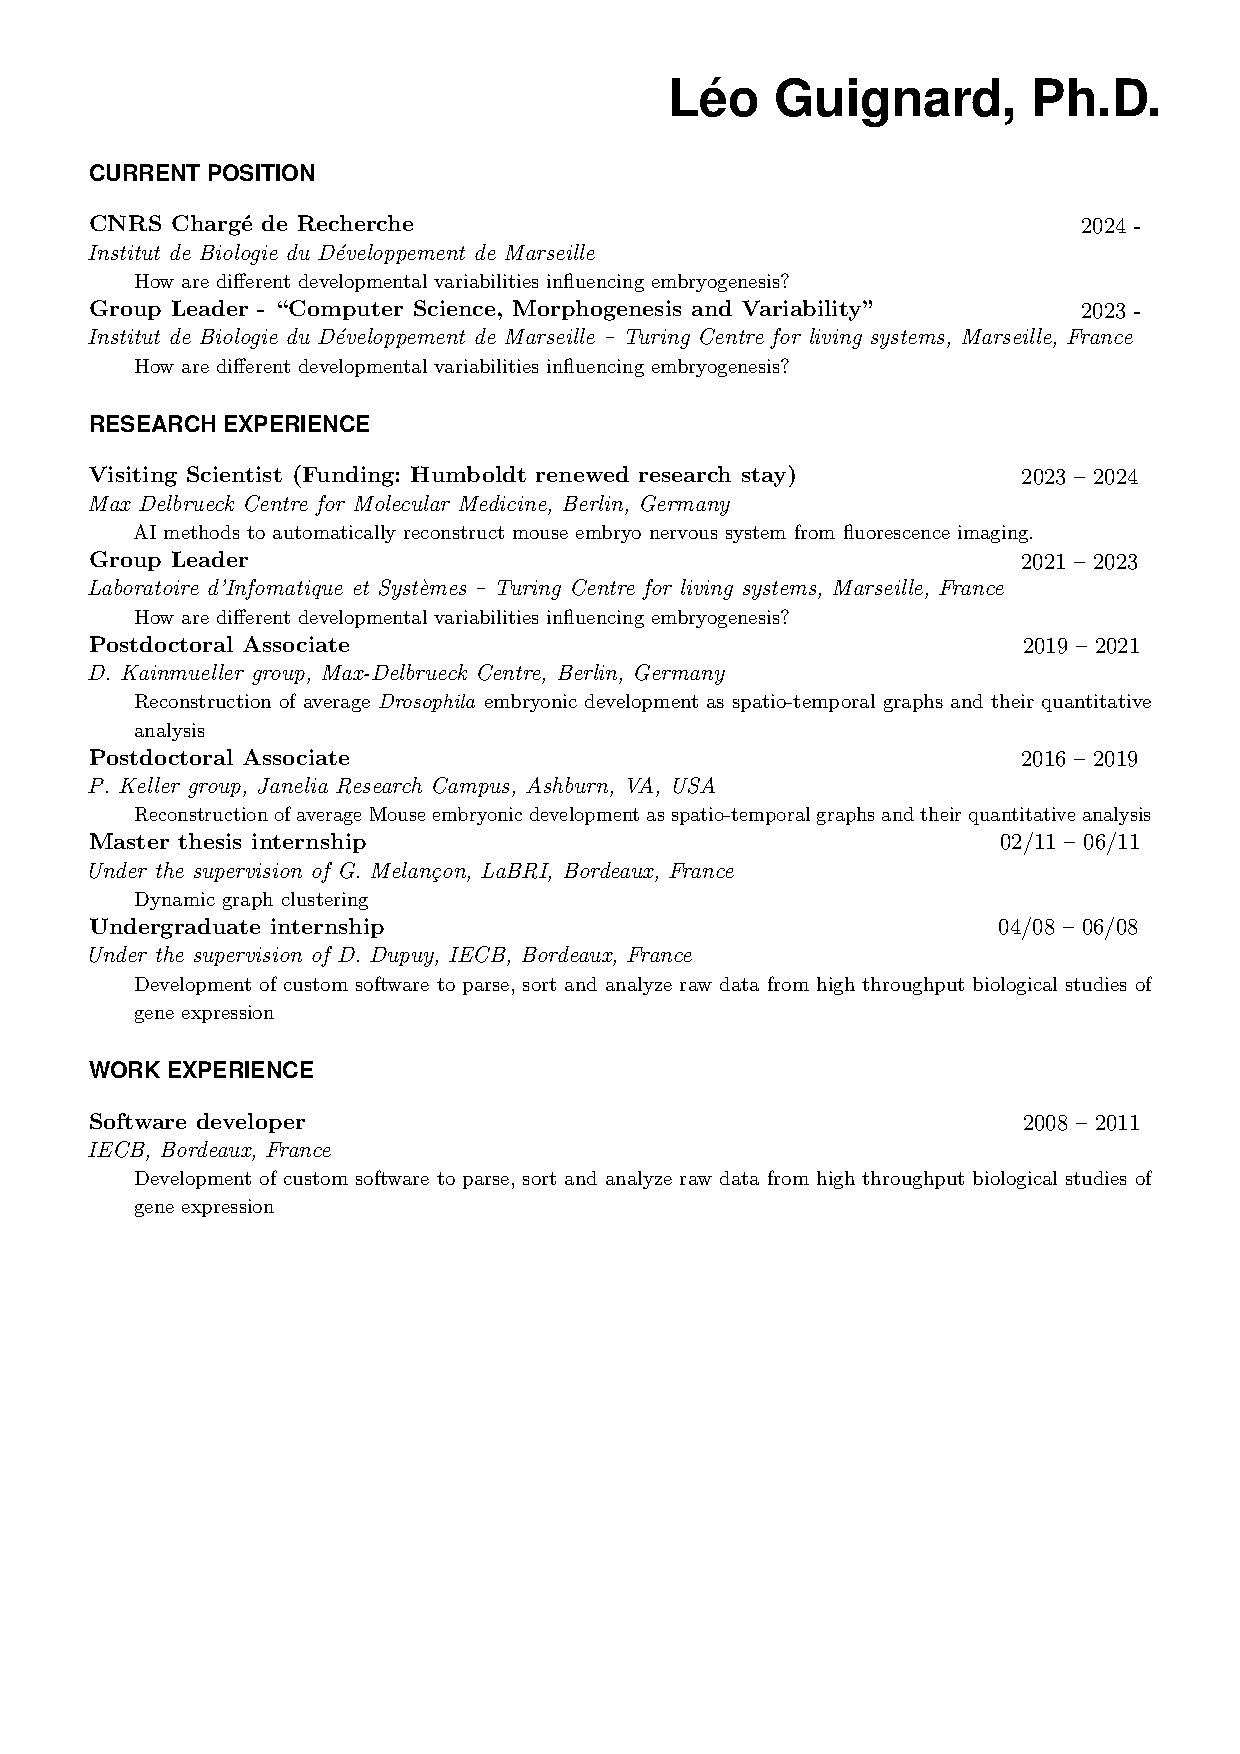
\includepdf[
	pages=1,
	scale=0.85,
	offset=0 25pt,
	pagecommand={%
		\cvpagestyle
		\phantomsection
		\addcontentsline{toc}{chapter}{\protect\nonumberline Curriculum vitae}%
		\label{chap:cv}%
		},
	]{guignard-leo-cv.pdf}

%% pages suivantes
\includepdf[
	pages=2-,
	scale=0.85,
	offset=0 25pt,
	pagecommand={\cvpagestyle},
	]{guignard-leo-cv.pdf}
